\documentclass[a4paper]{article}

%% Language and font encodings
\usepackage[english]{babel}
\usepackage[utf8x]{inputenc}
\usepackage[T1]{fontenc}

%% Sets page size and margins
\usepackage[a4paper,top=3cm,bottom=2cm,left=3cm,right=3cm,marginparwidth=1.75cm]{geometry}

%% Useful packages
\usepackage{amsmath}
\usepackage{graphicx}
\usepackage[colorinlistoftodos]{todonotes}
\usepackage[colorlinks=true, allcolors=blue]{hyperref}
\usepackage{algorithm2e}
\usepackage{hyperref}
\usepackage{listings}
\usepackage{pgfplots}
\pgfplotsset{compat=1.14}

\setlength{\parindent}{0pt}


\title{Applications of Data Analysis 2018\\Excercise 4\\\emph{Predicting water permeability exponent with SKCV}}
\author{Timo Heinonen\\509445\\tijuhe@utu.fi}

\begin{document}
\fontfamily{\sfdefault}\selectfont
\maketitle

\section{Description of the problem}
The goal of this data analysis task was to predict water permeability of soil from a number of measured attributes. Three data files were provided; \emph{inputs} contained 1691 rows of numerical feature values, \emph{outputs} contained the corresponding water permeability exponents and \emph{coordinates} contained 2-dimentional meter coordinates of the measurement points.\\

The task was to use the k-nearest-neighbors algorithm with leave-one-out spatial cross-validation and evaluate the model with the c-index. I was able to use quite a lot of code written for previous exercises.\\

Because measurement points that are close together usually have quite similar types of soil, the data contains strong correlations between nearby points. This is why spatial cross-validation was used. The division of the data to test and training sets was done so that measurements whose distance to the test object was less than a predefined $\delta$ were rejected from the training set.


\section{Process}
Below is described the work I did in order to create a model for the problem and evaluate it. Please note that the complete source code with comments is presented at the end of this document.

\begin{itemize}
\item First I opened and parsed the three data files and standardized the inputs with z-score:


\fontfamily{pcr}\selectfont
\footnotesize
\begin{lstlisting}
FILE_INPUTS = "data/permeability/input.csv"
FILE_OUTPUTS = "data/permeability/output.csv"
FILE_COORDINATES = "data/permeability/coordinates.csv"

inputs = open_and_parse(FILE_INPUTS)
outputs = open_and_parse(FILE_OUTPUTS)
coordinates = open_and_parse(FILE_COORDINATES)

inputs_std = stats.zscore(inputs)
\end{lstlisting}
\normalsize
\fontfamily{\sfdefault}\selectfont

\item Then I made nearest neighbor predictions with $k = 1,3,5,7,9$ and $\delta = 0, 10, 20, ...,200$. This took hours when using my unoptimized knn-functions. It turned out that the best values for $k$ were $9$ when $\delta < 100$ and $7$ when $\delta \geq 100$.
\fontfamily{pcr}\selectfont
\footnotesize
\begin{lstlisting}
ds_to_test = range(0, 201)[0::10]
ks_to_test = [1, 3, 5, 7, 9]
for d in ds_to_test:
    
    c_ixs = []
    for num_neighbors in ks_to_test:    
        prediction_func = partial(knn.predict_regression, k=num_neighbors)
        c_ix = spatial_loo_cv(inputs_std, outputs, coordinates, d, prediction_func)
        c_ixs.append(c_ix)
        print("d = " + str(d) + "k = " + str(num_neighbors) + ", C-index = " + str(c_ix))
\end{lstlisting}
\normalsize
\fontfamily{\sfdefault}\selectfont

\item The spatial leave-one-out cross-validation was implemented by simply not adding the nearby measurements to the training set: 
\fontfamily{pcr}\selectfont
\footnotesize
\begin{lstlisting}
def get_nearby_pnt_indices(pnts, ix_pnt, coordinates, delta):
    ixs = []
    for ix_other_pnt, item in enumerate(pnts):
        dist = knn.distance(coordinates[ix_pnt], coordinates[ix_other_pnt])

        if dist < delta:
            ixs.append(ix_other_pnt)

    return(ixs)


def spatial_loo_cv(inputs, outputs, coordinates, delta, f_predict):
    predictions = []
    for test_ix, test_inputs in enumerate(inputs):
        nearby_pnt_ixs = get_nearby_pnt_indices(inputs, test_ix, coordinates, delta)

        #Remove data of nearby points
        training_outputs = []
        training_inputs = []
        for ix, item in enumerate(inputs): 
            if (ix != test_ix) and (ix not in nearby_pnt_ixs):
                training_inputs.append(inputs[ix])
                training_outputs.append(outputs[ix])

        #Make prediction for test set
        prediction = f_predict([test_inputs], training_inputs, training_outputs)
        predictions.append(prediction)

    return(knn.c_index(outputs, predictions))
\end{lstlisting}
\normalsize
\fontfamily{\sfdefault}\selectfont



\item Finally I recomputed the c-indices for the best values of $k$ and the different values of $\delta$, and plotted a graph. The graph is presented in the next section:
\fontfamily{pcr}\selectfont
\footnotesize
\begin{lstlisting}
c_ixs = []
for d in ds_to_test:
    best_k = int()

    if d < 100:
        best_k = 9
    else: 
        best_k = 7
    
    prediction_func = partial(knn.predict_regression, k=best_k)

    c_ix = spatial_loo_cv(inputs_std, outputs, coordinates, d, prediction_func)
    c_ixs.append(c_ix)
	print("k = " + str(best_k) + ", delta = " + str(d) + ", C-index = " + str(c_ix))

print("Average C-index for the best values of k: " + str(mean(c_ixs)))

plt.plot(ds_to_test, c_ixs)
plt.xlabel('Delta')
plt.ylabel('C-index')
plt.title('C-indices with the best values of k for delta = 0, 10, ..., 200')
plt.xticks(range(0, 200, 20))
plt.show()
plt.savefig("c_idx_plot.png")
\end{lstlisting}
\normalsize
\fontfamily{\sfdefault}\selectfont
\end{itemize}

\newpage
\section{Results}

The model performance was rather poor with c-indices ranging from 0.5828 to 0.7224. The higher values were achieved with low delta and thus are biased. As expected, the c-index decreased when delta increased. Average c-index for the best values of $k$ was 0.6657. Table 1 shows the average c-index values for all values of $k$. Figure 1 was generated in the code and shows the c-indices for the best values of $\delta$.


\begin{table}[htp]
\begin{center}
\begin{tabular}{l|l}
$\delta$ & Average C-index  \\\hline
0&0.7084\\
10&0.7095\\
20&0.6978\\
30&0.6981\\
40&0.6950\\
50&0.6915\\
60&0.6860\\
70&0.6836\\
80&0.6795\\
90&0.6780\\
100&0.6768\\
110&0.6400\\
120&0.6206\\
130&0.6119\\
140&0.6108\\
150&0.6079\\
160&0.6077\\
170&0.6077\\
180&0.6071\\
190&0.6064\\
200&0.6058\\
\end{tabular}
\caption{\textbf{Average} c-index values for $k = 1,3,5,7,9$}
\end{center}
\end{table}



\begin{figure}
\begin{center}
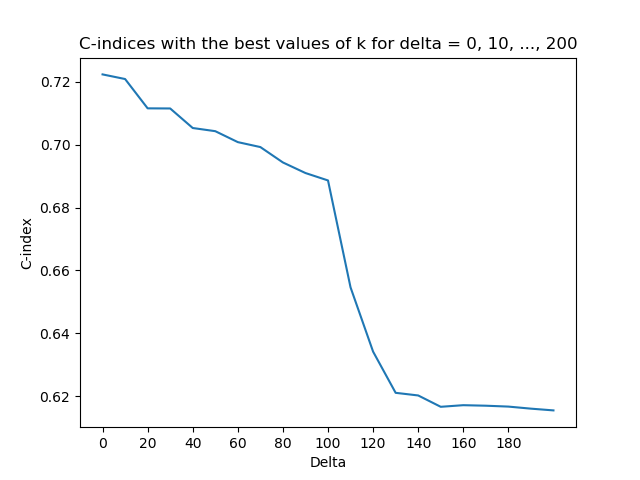
\includegraphics[width=0.8\textwidth]{c_idx_plot.png}
\caption{Plot drawn with the Python library \emph{matplotlib}}
\end{center}
\end{figure}


\newpage
\section{Source code}
Below is listed the source code of the program. For syntax highlighting, please visit my \href{https://github.com/jootimo/ml_repo}{GitHub page}. File $\href{https://github.com/jootimo/ml_repo/blob/master/water_permeability.py}{water\_permeability.py}$ handles the parsing of the data file, standardization, cross-validations, calling the knn-utilities and drawing the plot. $\href{https://github.com/jootimo/ml_repo/blob/master/knn.py}{knn.py}$ was written for the previous exercises and contains utilities for the k nearest neighbors algorithm.\\

I used some external libraries:
\begin{itemize}
\item \emph{math} for square root
\item \emph{operator} for sorting a list on values of one index
\item \emph{partial} for function argument binding
\item \emph{stats} for z-score standardization
\item \emph{matplotlib} for plotting
\end{itemize}

\vspace*{1cm}

\renewcommand{\sfdefault}{pcr}
\fontfamily{pcr}\selectfont

\textbf{water\_permeability.py:}\\
\footnotesize
\begin{lstlisting}
import knn                      # K-nearest-neighbors utilities
from functools import partial   # Function argument binding
from numpy import mean          # mean
from scipy import stats         # z-score

import matplotlib 
matplotlib.use('pdf')
import matplotlib.pyplot as plt #Plotting results

def open_and_parse(filename):
    ''' Open file with name filename and parse comma separated values a into 2-d list
        
        @param    filename
    '''
    data = []

    with open(filename, "r") as filestream:

        for line in iter(filestream.readline, ''):
            line = list(line.split(','))

            #Parse rows into lists
            for i in range(0, len(line)):

                #Remove newline characters
                line[i].replace('\n', '')

                line[i] = float(line[i])

            data.append(line)

    return data


def get_nearby_pnt_indices(pnts, ix_pnt, coordinates, delta):
    ''' Get indices of points in pnts that are close to the specified point

        @param    pnts        List of data points
        @param    ix_pnt      Index of the point in pnts to compare to
        @param    coordinates 2d Coordinates of the pnts
        @param    delta       Max distance of what is considered 'nearby'
    '''
    ixs = []
    for ix_other_pnt, item in enumerate(pnts):
        dist = knn.distance(coordinates[ix_pnt], coordinates[ix_other_pnt])

        if dist < delta:
            ixs.append(ix_other_pnt)

    return(ixs)



def spatial_loo_cv(inputs, outputs, coordinates, delta, f_predict):
    '''
    Perform spatial leave-one-out cross-validation for data and call a
    prediction function.

    @param  inputs      2d list of the input data
    @param  outputs     1d list of the corresponding outputs
    @param  coordinates List of 2d coordinates of where the measurements were made
    @param  delta       Size of the dead zone. Same unit as in coordinates
    @param  f_predict   Function used to make the predictions

    @return C-index value of the predictions
    '''

    predictions = []
    for test_ix, test_inputs in enumerate(inputs):
        nearby_pnt_ixs = get_nearby_pnt_indices(inputs, test_ix, coordinates, delta)

        #Remove data of nearby points
        training_outputs = []
        training_inputs = []
        for ix, item in enumerate(inputs): 
            if (ix != test_ix) and (ix not in nearby_pnt_ixs):
                training_inputs.append(inputs[ix])
                training_outputs.append(outputs[ix])

        #Make prediction for test set
        prediction = f_predict([test_inputs], training_inputs, training_outputs)
        predictions.append(prediction)

    return(knn.c_index(outputs, predictions))



######### Actual script ##########
FILE_INPUTS = "data/permeability/input.csv"
FILE_OUTPUTS = "data/permeability/output.csv"
FILE_COORDINATES = "data/permeability/coordinates.csv"

inputs = open_and_parse(FILE_INPUTS)
outputs = open_and_parse(FILE_OUTPUTS)
coordinates = open_and_parse(FILE_COORDINATES)

#Standardize inputs with z-score
inputs_std = stats.zscore(inputs)

#Test with delta values 0, 10, 20, ..., 200
ds_to_test = range(0, 201)[0::10]


'''
#Test nearest neighbors regression for different values of k
#and delta to find out the best values for k
ks_to_test = [1, 3, 5, 7, 9]
for d in ds_to_test:

    print("delta = " + str(d))

    c_ixs = []
    for num_neighbors in ks_to_test:    
        prediction_func = partial(knn.predict_regression, k=num_neighbors)

        c_ix = spatial_loo_cv(inputs_std, outputs, coordinates, d, prediction_func)
        print("k = " + str(num_neighbors) + ", C-index = " + str(c_ix))
        c_ixs.append(c_ix)
    
    print("Average C-index for delta = " + str(d) + ": " + str(mean(c_ixs)))
'''

#Best c-index values were achived when using k = 9 for delta < 100 and
#k = 7 for 100 <= delta <= 200
#
#Do predictions again, but this time only with the best k. Plot the 
#resulting c-indices.
c_ixs = []
for d in ds_to_test:
    best_k = int()

    if d < 100:
        best_k = 9
    else: 
        best_k = 7
    
    prediction_func = partial(knn.predict_regression, k=best_k)

    c_ix = spatial_loo_cv(inputs_std, outputs, coordinates, d, prediction_func)
    print("k = " + str(best_k) + ", delta = " + str(d) + ", C-index = " + str(c_ix))
    c_ixs.append(c_ix)


print("Average C-index for the best values of k: " + str(mean(c_ixs)))

plt.plot(ds_to_test, c_ixs)
plt.xlabel('Delta')
plt.ylabel('C-index')
plt.title('C-indices with the best values of k for delta = 0, 10, ..., 200')
plt.xticks(range(0, 200, 20))
plt.show()
plt.savefig("c_idx_plot.png")
\end{lstlisting}

\vspace*{1cm}
\normalsize
\textbf{knn.py:}\\
\footnotesize
\begin{lstlisting}
from math import sqrt
from operator import itemgetter
from numpy import mean


def distance(a, b):
    ''' Calculate the Euclidean distance between data points a and b
        
        @param    a   list of attribute values
        @param    b   list of attribute values

        @return   distance between a and b or -1 if lists have different lenghts 
    '''
    len_a = len(a)
    len_b = len(b)

    if len_a != len_b:
        return(-1)
    else:
        dist = 0
        for i in range(0, len_a):
            dist += (a[i] - b[i]) ** 2

        return sqrt(dist)


def compute_distances(test_data, training_data):
    ''' Compute distances from each data point in training data to that in test data

        @param    training_data  list of numerical data rows, excluding the attribute to predict
        @param    test_data      list of the data object to calculate distances to

        @return   distance list
    '''

    distances = []
    
    for i in range(0, len(test_data)):
        row = []
        for j in range(0, len(training_data)):
            dist = distance(test_data[i], training_data[j])
            row.append(dist)

        distances.append(row)

    return(distances)


def compute_nearest_neighbors(test_data, training_data, num_neighbors):
    ''' Compute nearest neighbors of the given data object

        @param    test_data       data object to compute distances to
        @param    training_data   data that the distances are computed to
        @param    num_neighbors   value of k

        @return   Indices of num_neighbors nearest neighbors of test_data in training_data
    '''

    #Compute distances to test_data
    distances = compute_distances(test_data, training_data)
    neighbors = []
    for ix_test_obj in range(0, len(test_data)):
        #Iterate over the distance list and create list of (row index, distance) pairs
        ixs_and_distances = []
        for i in range(0, len(distances[ix_test_obj])):
            ixs_and_distances.append([ i, distances[ix_test_obj][i] ])

        #Sort the list on distances and include only first num_neighbors elements
        ixs_and_distances.sort(key = itemgetter(1))
        k_nearest = ixs_and_distances[0 : num_neighbors]

        #Only return neighbor indices in training_data
        neighbors_of_row = []
        for n in k_nearest:
            neighbors_of_row.append(n[0])

        neighbors.append(neighbors_of_row)

    return(neighbors)


def predict_regression(test_inputs, training_inputs, training_outputs, k):
    ''' Predict an output for an input based it's the nearest neighbors

        @param    test_inputs         Inputs to predict an output for
        @param    training_inputs     Data to calculate neighbors from
        @param    training_outputs    True outputs for training_inputs
        @param    k                   Number of neighbors to use

        @return   Mean value of k nearest neighbors
    '''
    neighbor_ixs = compute_nearest_neighbors(test_inputs, training_inputs, k)
        
    neighbor_outputs = []
    for i in neighbor_ixs[0]:
        neighbor_outputs.append(training_outputs[i])

    prediction = mean(neighbor_outputs)

    return(prediction)
\end{lstlisting}


\end{document}